% Nama Kelompok : Kelompok 4
% Akbar Pambudi Utomo (1154094) 
% Andi Nurfadilah Ali (1154041)
% Andi Wadi Afryandika (1154113)
% Hanna Theresia Siregar (1154009)
% Julham Ramadhana (1154069)
% Pebridayanti Hasibuan (1154118)

\section{Sejarah Bumi}
Bumi merupakan planet atau rumah kita dalam kedudukan di tata surya. peradaban kuno percaya bahwa bumi itu datar, dengan langit berputar-putar sekali sehari. secara umum yang diyakini bahwa kehidupan di Bumi dimulai di Bumi itu sendiri, beberapa waktu setelah terbentuknya planet antara 4000-5000 juta tahun yang lalu. namun ada yang berpendapat bahwa kehidupan diluar bumi itu ada, tetap kita tidak memiliki bukti pasti tentang kehidupan di tempat lain. yang perlu kita ketahui bumi berada pada galaksi bimasakti dimana terdapat matahari sebagai sistem bintang.
Dalam Geologi sendiri atau biasa disebut sebagai ilmu pengetahuan tentang Kebumian yang mempelajari segala sesuatu mengenai planet Bumi beserta isinya yang pernah ada. Dalam Geologi juga akan dibahas tentang sifat-sifat dan bahan- bahan yang membentuk bumi itu apa, serta struktur dan proses-proses yang bekerja baik didalam maupun dibagian teratas permukaan bumi, kedudukannya di Alam Semesta hingga sekarang. Geologi merupakan ilmu pengetahuan yang komplek, mempunyai pembahasan materi yang beraneka ragam namun juga merupakan ilmu pengetahuan yang enak dipelajari. Sebagai landasan prinsip untuk dapat mempelajari ilmu geologi adalah bahwasanya kita harus menganggap bumi ini sebagai suatu benda yang secara dinamis berubah sepanjang masa, setiap saat dan setiap detik. 
Pemikiran geologi modern dikenalkan oleh Huttonian revolution mengemukakan pemikiran-pemikirannya sebagai berikut:
1. Bahwasanya proeses-proses alam yang sekarang ini menyebabkan perubahan pada permukaan bumi, juga bekerja sepanjang umur dari bumi ini. 
2. Ia juga mengamati bahwa proses-proses tersebut yang walaupun bekerja sangat lambat, tetapi pada akhirnya mampu menyebabkan terjadinya perubahan-perubahan yang sangat besar pada bumi. 
3. Bahwa bumi ini sangat dinamis, yang berarti mengalami perubahan-perubahan yang terus-menerus mengikuti suatu pola daur (siklus) yang berulang-ulang.
Bumi sendiri berada di kawasan dimana terjadinya tumpang tindih antara litosfer (daratan) bagian padat dari bumi, hidrosfer (perairan), dan atmosfer (udara) yang menyelubungi bumi dengan zarah-zarah dan benda-benda yang mengisinya.
Dalam sejarah terbentuknya bumi sewaktu SMA kita pernah mempelajari teori-teori terbentuknya bumi dalam pelajaran geografi.\cite{wetherill1990formation}

\subsection{Teori-teori terbentuknya Bumi}
\subsubsection{1.Teori Kabut Kant-Laplace}
\begin{figure} [ht]
	\centerline{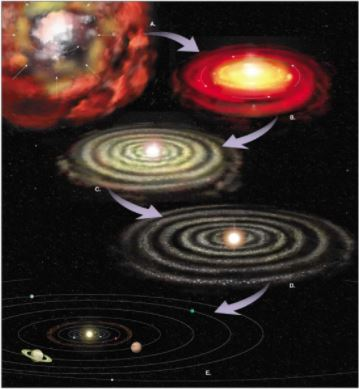
\includegraphics[width=1\textwidth]{figures/teorikabutnebula.JPG}}
	\caption{Gambar Teori Nebula}
	\label{teorikabutnebula}
	\end{figure}
	Pada Gambar berikut \ref{teorikabutnebula} adalah gambar dari Teori Kabut Nebula.
Teori ini dikenal dengan teori kabut (nebula) yang dikemukakan oleh Immanuel Kant (1755) dan Pierre de Laplace (1796). dalam teori ini dikemukakan bahwa di jagat raya terdapat gas yang kemudian berkumpul menjadi kabut(nebula). gaya tarik-menarik antargas ini membentuk kumpulan kabut yang sangat besar dan berputas semakin cepat sehingga materi kabut bagian khatulistiwa terlempar memisah dan memadat(karena pendinginan), bagian yang terlempar inilah yang kemudian menjadi sebuah planet dalam tatasurya. Bumi baru terus bertumbuh sampai suhu interiornya cukup panas untuk melelehkan logam siderofil. Dengan massa jenis yang lebih tinggi dari silikat, akhirnya logam ini tenggelam. Proses ini terjadi 10 juta tahun setelah Bumi mulai terbentuk, dan menghasilkan struktur Bumi yang berlapis-lapis dan mengakibatkan terbentuknya medan magnet. J. A. Jacobs merupakan orang pertama yang menunjukkan bahwa inti dalam—bagian dalam yang padat berbeda dari inti luar yang padat—membeku dan mengembang keluar inti luar yang cair dikarenakan bagian dalam bumi yang makin mendingin (sekitar 100° C per miliar tahun. Ekstrapolasi dari pengamatan ini memperkirakan bahwa inti terbentuk pada masa 2–4 miliar tahun yang lalu. Jika ini benar maka berarti bahwa inti bumi bukanlah fitur primordial yang berasal selama pembentukan planet.

\subsubsection{2.Teori Planetesimal}
\begin{figure} [ht]
	\centerline{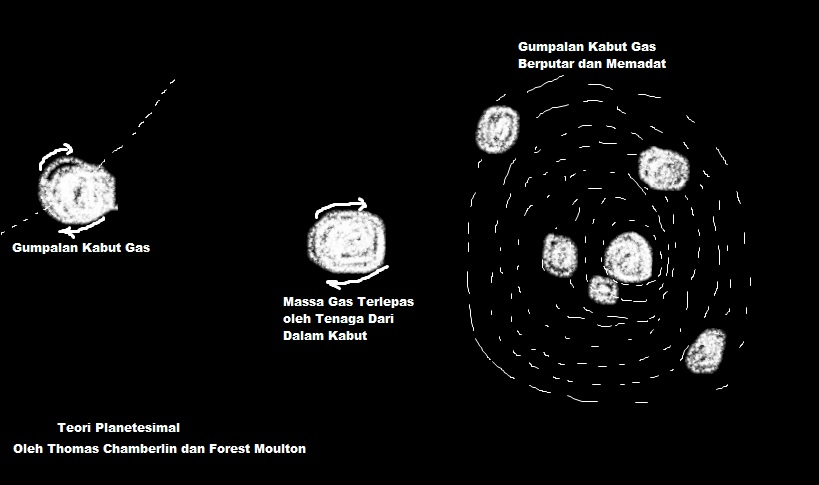
\includegraphics[width=1\textwidth]{figures/teoriplanetesimal.JPG}}
	\caption{Gambar Teori Planetesimal}
	\label{teoriplanetesimal}
	\end{figure}
	Pada Gambar berikut \ref{teoriplanetesimal} adalah gambar dari Teori Planetesimal.
seabad kemudian sesudah teori kabut tersebut muncul teori Planetesimal yang dikemukakan oleh Chamberlin dan Moulton. Teori ini mengungkapkan bahwa pada mulanya telah terdapat Matahari asal. pada suatu ketika, matahari asal ini didedakti sebuah bintang besar yang menyebabkan terjadinya penarikan pada bagian matahari. Akibat tenaga tarik menarik tadi, terjadilah ledakan yang dasyat. Gas yang meledak ini keluar dari atmosfer matahari, kemudian mengembun dan membeku sebagai benda-benda yang padat(disebut planetesimal). Planetesimal ini dalam perkembangannya menjadi planet-planet, dan salah satunya planet bumi kita.

\subsubsection{3.Teori Pasang Surut Gas}
\begin{figure} [ht]
	\centerline{\includegraphics[width=1\textwidth]{figures/teoripasangsurut.JPG}}
	\caption{Gambar Pasang Surut}
	\label{teoripasangsurut}
	\end{figure}
	Pada Gambar berikut \ref{teoripasangsurut} adalah gambar dari Teori Pasang Surut.
Teori ini dikemukakan oleh Jeans dan Jeffreys, yakni bahwa sebuah bintang besar mendekati matahari dalam jarak pendek, sehingga menyebabkan terjadinya pasang surut pada tubuh matahari. dalam lidah yang panas ini terjadi perapatan gas-gas dan akhirnya kolom-kolom ini akan pecah, lalu berpisah menjadi benda-benda tersendiri yaitu planet-planet. bintang besar yang menyebabkan penarikan pad abagian-bagian tubuh matahari tadi melanjutkan perjalanan di jagat raya, sehingga lambat laun akan hilang pengaruhnya terhadapt planet-planet yang terbentuk tadi, lalu planet-planet itu akan mengelilingi matahari dan mengalami proses pendinginan, proses pendinginan berjalan lambat pada planet besar seperti yupiter dan saturnus, sedangkan planet kecil seperti bumi mengalami proses pendinginan yang relatif lebih cepat.

\subsubsection{4. Teori Bintang Kembar}
\begin{figure} [ht]
	\centerline{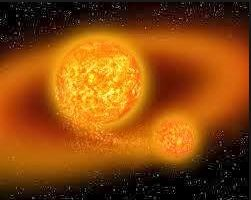
\includegraphics[width=1\textwidth]{figures/teoribintangkembar.JPG}}
	\caption{Gambar Teori Bintang Kembar}
	\label{teoribintangkembar}
	\end{figure}
	Pada Gambar berikut \ref{teoribintangkembar} adalah gambar dari Teori Bintang Kembar.
Teori ini dikemukakan oleh seorang ahli astronomi R. A. Lyttleton. Menurut teori ini, galaksi berasal dari kombinasi bintang kembar. Salah satu bintang meledak sehingga banyak materi yang terlempar. Karena bintang yang tidak meledak mempunyai gaya gravitasi yang masih kuat, maka sebaran pecahan ledakan bintang tersebut mengelilingi bintang yang tidak meledak. Bintang yang tidak meledak itu adalah matahari, sedangkan pecahan bintang yang lain itu adalah planet-planet yang mengelilinginya.

\subsubsection{5. Teori Dentuman Besar (Big Bang Teory)}
\begin{figure} [ht]
	\centerline{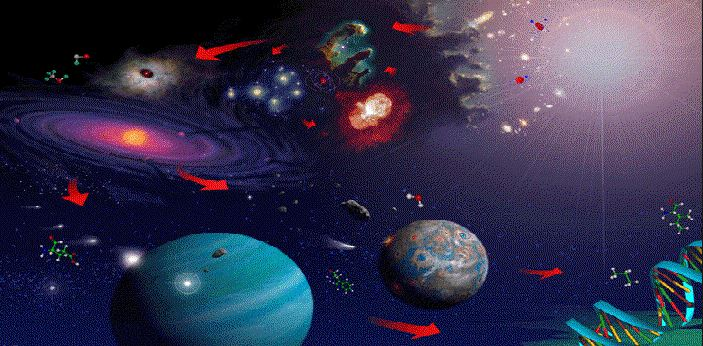
\includegraphics[width=1\textwidth]{figures/teoribigbang.JPG}}
	\caption{teoribigbang}
	\label{teoribigbang}
	\end{figure}
	Pada Gambar berikut \ref{teoribigbang} adalah gambar dari Teori Dentuman Besar(BigBang).
Pada Teori ini berdasarkan dari asumsi adanya massa yang sangat besar dan mempunyai massa jenis sangat besar. Adanya reaksi inti menyebabkan massa tersebut meledak hebat. Massa tersebut kemudian mengembang dengan sifat sangat cepat menjauhi pusat ledakan, karena danya gravitasi, maka bintang yang paling kuat gravitasinya akan menjadi pusatnya.
Dari berbagai teori, teori ini yang paling banyak didukung oleh para ilmuwan.

\section{Pendapat Tentang Sejarah Bumi}
Bumi terbentuk sekitar 4,54 miliar (4,54×109) tahun yang lalu melalui akresi dari nebula matahari. Pelepasan gas vulkanik diduga menciptakan atmosfer tua yang nyaris tidak beroksigen dan beracun bagi manusia dan sebagian besar makhluk hidup masa kini. Sebagian besar permukaan Bumi meleleh karena vulkanisme ekstrem dan sering bertabrakan dengan benda angkasa lain. Sebuah tabrakan besar diduga menyebabkan kemiringan sumbu Bumi dan menghasilkan Bulan. Seiring waktu, Bumi mendingin dan membentuk kerak padat dan memungkinkan cairan tercipta di permukaannya. Bentuk kehidupan pertama muncul antara 2,8 dan 2,5 miliar tahun yang lalu. Kehidupan fotosintesis muncul sekitar 2 miliar tahun yang lalu, nan memperkaya oksigen di atmosfer. Sebagian besar makhluk hidup masih berukuran kecil dan mikroskopis, sampai akhirnya makhluk hidup multiseluler kompleks mulai lahir sekitar 580 juta tahun yang lalu. Pada periode Kambrium, Bumi mengalami diversifikasi filum besar-besaran yang sangat cepat. Perubahan biologis dan geologis terus terjadi di planet ini sejak terbentuk. Organisme terus berevolusi, berubah menjadi bentuk baru atau punah seiring perubahan Bumi. Proses tektonik lempeng memainkan peran penting dalam pembentukan lautan dan benua di Bumi, termasuk kehidupan di dalamnya. Biosfer memiliki dampak besar terhadap atmosfer dan kondisi abiotik lainnya di planet ini, seperti pembentukan lapisan ozon, proliferasi oksigen, dan penciptaan tanah.Dalam sebuah artikel dari zuhdi2012sistem yang menyebutkan bahwa Bumi merupakan salah satu planet yang berada dalam tata surya yang diduga terbentuk dari pecahan-pecahan bintan pada jutaan tahun yang lalu, dan kemudian terperangkapa pada gravitasi matahari sehinggan akan selalu mengelilingi matahari. Menurut Hukum Newton kenapa planet dapat bertahan dalam pergerakan keliling atau biasa disebut revolusi dikarenakan planet melakukan gerak melingkar yang menimbulkan gaya sentifugal yang besarnya  dengan gaya gravitasi namun berlawanan arah. Gaya gravitasi ini sendiri akan berkurang sesuai dengan semakin jauhnya jarak planet dari matahari, sedangkan gaya sentrifugal  akan tergantung pada kecepatan gerak melingkar planet. Semakin cepat gerakan tersebut maka akan semakin besar daya sentifugal. Bila secara kebetulan kedua gaya ini memiliki kecepatan yang sama besar, maka planet akan terjebak mengelilingi matahari. Pada saat tata surya terbentuk diperkirakan terdapat jutaan planet. Akan tetapi sebagian terjatuh ke matahari atau terlempar lepas dari pengaruh matahari. Selain berkeliling, planet juga akan bergerak memutari pororsnya (rotasi). Gerak rotasi ini sendiri berlangsung dalan waktu lama sehingga membuat planet berbentuk seperti bola. Pada masa lalu, planet planet bukanlah sebuah benda padat, melainkan berupa magma atau berupa cairan batu. Bagian padat pada planet terbentuk selama proses pendinginan dan terjadi pada bagian kulit terluar dari planet tersebut. Bentuk Bumi sendiri yang dikatakan berbentuk bola tidakalah sempurna. Gerak Rotasi telah mengubah bentuk bumi menjadi agak cepat terhadap kedua kutubnya.\cite{zuhdi2012sistem}


Sejarah pembentukan Bumi yang dipelajari dalam materi pelajaran Geografi cenderung memiliki sifat abstrak yang akan lebih mudah dimengerti, jika memakai media yang cocok. Salah satu Inovasi pembelajaran yang tepat untuk dilakukan adalah menggunakan kartu indeks dan media film. Media seperti kartu indeks yang dipergunakan sebaga salah satu upaya yang memudahkan peserta didik agar mengingat konsep-konsep materi yang sedang dipelajari sedangkan media film sendiri merupakan media visual yang akan menjelaskan dengan lebih konkrit tentang fenomena bumi. Dalam sebuah artikel dari @article{widiyati2011meningkatkan menyebutkan bahwa Pmebentukan Bumi dengan kategori Continental Drift Theory atau biasa disebut dengan teori pengapungan benua yang dikemukan oleh Alfred Wegener pada tahun 1912 mengemukakan bahwa sampai sekitar 255 juta tahun lalu, di bumi baru ada satu benua dan samudera yang sangat luas. Benua raksasa ini sendiri dinamakan pangea, sedangkan kawasan samudera yang mengapitnya itu mengalami retakan-retakan dan pecah. Sekitar 135 juta tahun lalu, benua raksasa tersebut pecah menjadi dua, yaitu pecahan benua di sebelah utara yang dinamakan Lauransia dan dibagian selatan dinamakan gondwana.
\cite{widiyati2011meningkatkan}
